% -*- mode: latex-mode; TeX-engine: xetex; LaTeX-command-style: (("" "SOURCE_DATE_EPOCH=0 %(PDF)%(latex) --shell-escape %S%(PDFout)")); TeX-master: "../dissertation.tex"; -*-

\chapter{Loading of Single Atoms in Optical Tweezer}
\label{ch:loading}

\section{Introduction}
\label{ch:loading:introduction}

\section{Free Spacing Cooling of Atoms}
\label{ch:loading:free-space}

\begin{figure}
  \centering
  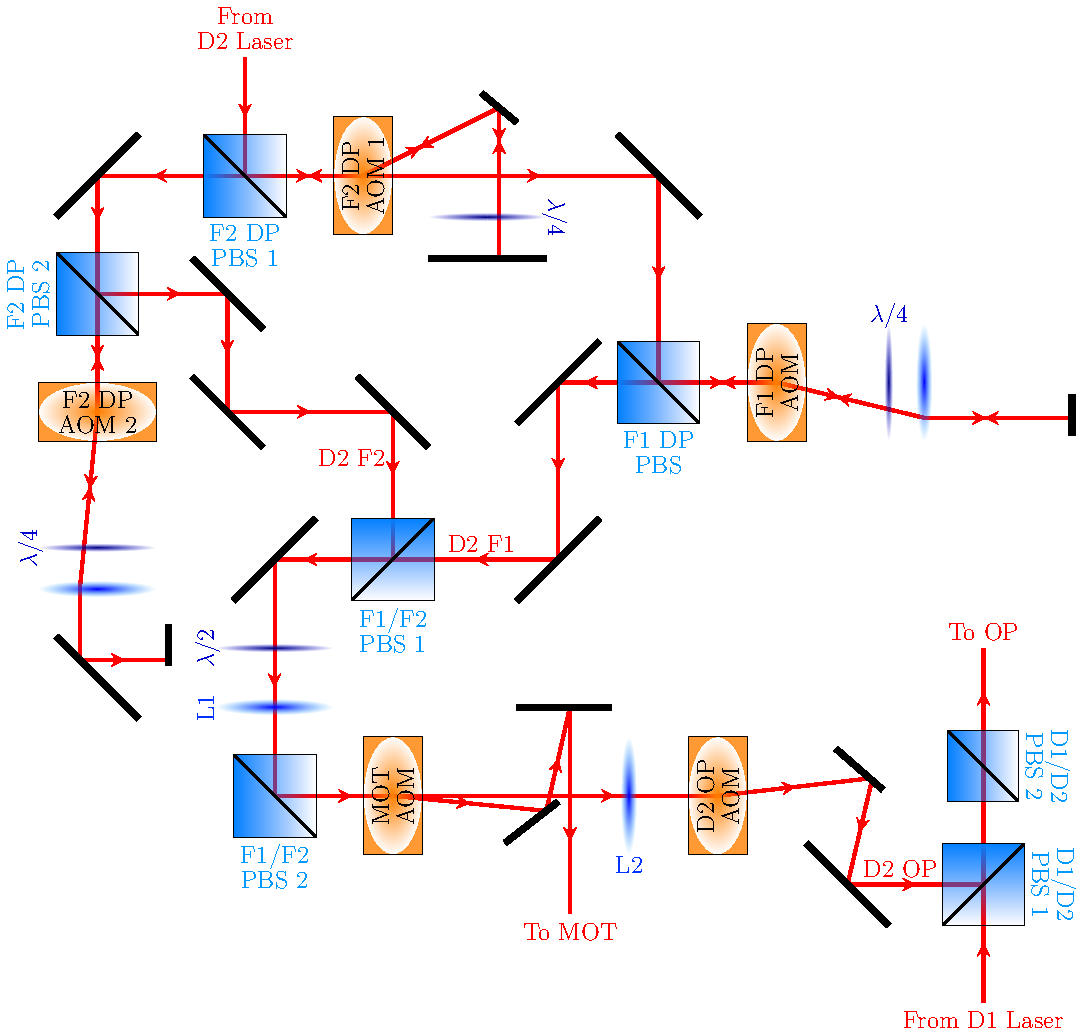
\includegraphics[width=\textwidth]{figures/loading_na_res_beampath.pdf}
  \caption[Beampath for Na D1 and D2 light.]{
    Beampath for generating the frequencies for Na MOT and optical pumping~(OP).
    (Beampath for fiber coupling and frequency locking is not shown.
    The power control for the D1 laser is also omitted.)
    The D2 laser is locked in the F1/F2 crossover line\todo{ref}.
    It is shifted down by the two F2 double-pass~(DP) AOMs to generate the frequency
    for the Na $F=2$ state and shifted up by the F1 DP AOM to address the Na $F=1$ state.
    The frequencies of the F1/F2 light are controlled by the F1 DP AOM
    and F2 DP AOM 2 respectively.
    This set up makes sure that when the F1/F2 DP AOMs are off,
    the closest frequency in the leaked light is at least detuned
    by half the F1/F2 separation~($\approx880~\mathrm{MHz}$)~\cite{steck_sodium_2019}
    and will have minimum effect on the atom.
    The F1 and F2 light are combined on F1/F2 PBS 1 and their power ratio after the
    F1/F2 PBS 2 is controlled by the half waveplate between the two PBSs.
    A similar setup is used to combine the D1 and D2 light in the OP output using
    D1/D2 PBS 1 and the rotating D1/D2 PBS 2.
    Since we need to switch the Na MOT light on and off out-of-phase
    with the Na tweezer~\cite{hutzler_eliminating_2017} at a high frequency,
    the sharpness of the turn on/off edge in the MOT AOM is important.
    We focus the beam through the AOM using lens L1 to optimize the switching time.
    This is then collimated by lens L2 for the downstream beampath.
    \label{fig:loading:free-space:na-res-beampath}}
\end{figure}

\ref{fig:loading:free-space:na-res-beampath}

\todo{
  MOT beam path
  MOT power balance
  Alignment
  Loading from background vapor
  CMOT
  Molasses
}

\section{Optical Tweezer}
\label{ch:loading:tweezer}

\todo{
  NA
  Beam path
}

\section{Loading and Imaging in the Tweezer}
\label{ch:loading:loading}

\todo{
  Light shift
  Live signal
  Loading
}

\section{Summary and Outlook}
\label{ch:loading:summary}
